%=============================================================================
%  GEMA — Gemelo Digital Metabólico   |   Artículo en formato IEEE
%  Universidad Nacional de Ingeniería (UNI) — FIIS
%  Formato apegado a "Anexo1_IEEE Artículo editable.docx":
%    US Letter · 2 columnas · Times New Roman · cuerpo 9pt · títulos romanos
%    centrados · subtítulos A./1) en cursiva · pies de figura y referencias 8pt
%=============================================================================
\documentclass[9pt,letterpaper,twocolumn]{extarticle}

\usepackage[utf8]{inputenc}
\usepackage[T1]{fontenc}
\usepackage[spanish,es-tabla,es-noindentfirst]{babel}
\usepackage{mathptmx}            % Times New Roman para texto y matemáticas
\usepackage{courier}             % Courier para los correos electrónicos
\usepackage{graphicx}
\usepackage{amsmath,amssymb}
\usepackage{booktabs}
\usepackage{array}
\usepackage{tabularx}
\usepackage{multirow}
\usepackage{caption}
\usepackage{float}
\usepackage{titlesec}
\usepackage{enumitem}
\usepackage{xcolor}
\usepackage{tikz}
\usetikzlibrary{shapes.geometric,arrows.meta,positioning,calc,fit,backgrounds}
\usepackage[colorlinks=true,linkcolor=black,citecolor=black,urlcolor=blue]{hyperref}
\usepackage{flushend}            % equilibra las columnas de la última página

% --- Geometría exacta del formato (carta US, márgenes del documento guía) ---
\usepackage[letterpaper,top=19mm,bottom=25.4mm,left=17.3mm,right=17.3mm,
            columnsep=4.22mm]{geometry}

% --- Sin números de página, encabezados ni pies (lo exige el formato) ---
\pagestyle{empty}

% --- Numeración: secciones en romano, tablas en romano ---
\renewcommand{\thesection}{\Roman{section}}
\renewcommand{\thesubsection}{\Alph{subsection}}
\renewcommand{\thesubsubsection}{\arabic{subsubsection})}
\renewcommand{\thetable}{\Roman{table}}

% --- Encabezados de sección al estilo IEEE ---
\titleformat{\section}[block]
  {\centering\normalsize\scshape}{\thesection.\;}{0.4em}{}
\titlespacing*{\section}{0pt}{2.4ex plus 1ex minus .2ex}{1.4ex plus .2ex}
\titleformat{\subsection}[block]
  {\normalsize\itshape}{\thesubsection.\;}{0.4em}{}
\titlespacing*{\subsection}{0pt}{1.8ex plus .6ex}{0.9ex}
\titleformat{\subsubsection}[runin]
  {\normalsize\itshape}{\thesubsubsection\;}{0.3em}{}[.]
\titlespacing*{\subsubsection}{\parindent}{0.6ex}{0.6em}

% --- Pies de figura y títulos de tabla a 8pt ---
\captionsetup{font=footnotesize,labelfont=bf,justification=justified,
              singlelinecheck=false,skip=4pt}
\captionsetup[figure]{name=Fig.,labelsep=period}
\captionsetup[table]{name=TABLA,labelsep=newline,justification=centering,
                     singlelinecheck=true,position=above,textfont={footnotesize,sc}}

\graphicspath{{figs/}}
\setlength{\parindent}{1.2em}
\setlength{\columnsep}{4.22mm}
\frenchspacing
\raggedbottom

\definecolor{gblue}{HTML}{2563EB}
\definecolor{ggreen}{HTML}{0E9F6E}
\definecolor{gpurple}{HTML}{7C3AED}
\definecolor{gink}{HTML}{111827}
\definecolor{gsoft}{HTML}{EEF2FF}
\definecolor{gsoft2}{HTML}{ECFDF5}
\definecolor{gsoft3}{HTML}{FAF5FF}
\definecolor{gsoft4}{HTML}{FFF7ED}

\begin{document}

%=============================================================================
% ENCABEZADO QUE ABARCA LAS DOS COLUMNAS
%=============================================================================
\twocolumn[{%
\begin{center}
{\fontsize{20}{24}\selectfont\bfseries
GEMA: Gemelo Digital Metabólico con Aprendizaje\\[2pt]
Automático para la Detección Temprana del\\[2pt]
Síndrome Metabólico en el Contexto Peruano}\\[14pt]

{\fontsize{11}{13}\selectfont
León Sánchez Fransua Mijail,\quad Escudero Díaz Alessandro Leonardo,\\[2pt]
Mejía Urbina Cristian Leonel,\quad Carhuamaca Rivera Stefany Miluska}\\[8pt]

{\fontsize{10}{12}\selectfont\itshape
Facultad de Ingeniería Industrial y de Sistemas\\
Universidad Nacional de Ingeniería --- Lima, Perú}\\[5pt]

{\fontsize{9}{11}\selectfont\ttfamily
fransua.leon.s@uni.pe\quad alessandro.escudero.d@uni.pe\\[1pt]
cristian.mejia.u@uni.pe\quad stefany.carhuamaca.r@uni.pe}
\end{center}
\vspace{10pt}
}]

%=============================================================================
% RESUMEN
%=============================================================================
\noindent\textbf{\textit{Resumen}---En el Perú casi nueve de cada diez adultos
cargan con alguna alteración metabólica, pero el síndrome metabólico avanza en
silencio porque no se detecta a tiempo ni se hace seguimiento: conseguir una
cita con un especialista del MINSA puede tomar entre dos y seis meses, y tratar
una diabetes ya declarada le cuesta al Estado entre S/\,3\,500 y S/\,8\,000 al
año por paciente. Presentamos GEMA, un gemelo digital que reconstruye el
comportamiento metabólico de cada persona a partir de un sensor continuo de
glucosa, un reloj inteligente y lo que la persona registra a diario, y resume
ese estado en un Índice de Carga Metabólica (ICM, 0--100) que da vida a un
avatar. El motor de inteligencia son dos modelos de aprendizaje automático
entrenados con una población sintética construida sobre relaciones fisiológicas
publicadas: un clasificador de riesgo (Random Forest) con 88,5\,\% de exactitud
(validación cruzada de 87,5\,\%$\pm$0,9\,\%) y un predictor del pico glucémico
postprandial (Gradient Boosting) con un error de 6,3\,mg/dL ($R^2=0{,}91$).
Ambos superan las metas que nos fijó la guía técnica del proyecto ($>$85\,\% y
$<$15\,mg/dL). Sobre el predictor montamos un simulador de escenarios
``¿qué pasaría si\ldots?'' del que salen recomendaciones concretas y medibles.
Todo esto se entrega en un MVP funcional de 14 pantallas. La motivación de fondo
es simple: no existe todavía un gemelo metabólico pensado para la dieta y el
perfil del adulto peruano.}

\vspace{4pt}
\noindent\textbf{\textit{Palabras clave}---}\textit{gemelo digital, síndrome
metabólico, aprendizaje automático, Random Forest, Gradient Boosting, predicción
glucémica, salud digital, Perú.}

%=============================================================================
\section{Introducción}
%=============================================================================
El síndrome metabólico es la antesala de buena parte de la carga de enfermedad
crónica del país. Reúne varias alteraciones que suelen aparecer juntas
---obesidad abdominal, glucosa elevada, triglicéridos altos, HDL bajo e
hipertensión--- y que comparten una raíz común: la resistencia a la insulina. Se
diagnostica cuando se cumplen al menos tres de los cinco criterios de la
Tabla~\ref{tab:criterios}~\cite{ncep}. Lo que vuelve peligrosa a esta condición
no es ninguno de esos criterios por separado, sino que durante años no produce
síntoma alguno. Para cuando la persona siente algo, el daño ya está hecho: el
camino habitual va de la alteración silenciosa a la prediabetes, de ahí a la
diabetes tipo 2 y, finalmente, a la enfermedad cardiovascular o renal.

\begin{table}[t]
\caption{Componentes diagnósticos del síndrome metabólico (a la vez, inputs del gemelo)}
\label{tab:criterios}
\footnotesize
\renewcommand{\arraystretch}{1.25}
\begin{tabularx}{\columnwidth}{@{}>{\raggedright\arraybackslash}X
                                >{\raggedleft\arraybackslash}p{3.7cm}@{}}
\toprule
\textbf{Componente} & \textbf{Umbral diagnóstico (H\,/\,M)}\\
\midrule
Circunferencia de cintura & $\geq$102 / $\geq$88\,cm \\
Triglicéridos             & $\geq$150\,mg/dL \\
Colesterol HDL            & $<$40 / $<$50\,mg/dL \\
Presión arterial          & $\geq$130/85\,mmHg \\
Glucosa en ayunas         & $\geq$100\,mg/dL \\
\bottomrule
\end{tabularx}
\end{table}

El sistema de salud actual llega tarde a este problema por tres razones que
identificamos al estudiar el contexto. La primera es el tiempo de espera: en el
MINSA, ver a un especialista puede demorar entre dos y seis meses, y la
enfermedad no espera. La segunda es la falta de seguimiento: una vez fuera del
consultorio, el paciente queda solo, sin retroalimentación ni alertas, lo que
explica las altas tasas de abandono del tratamiento. La tercera es el costo:
atender un caso de diabetes ya instalada cuesta entre S/\,3\,500 y S/\,8\,000
anuales por paciente, y las descompensaciones agudas evitables pueden disparar
ese gasto hasta en 239\,\%.

Las cifras dimensionan la urgencia (Fig.~\ref{fig:epi}). La prevalencia nacional
de síndrome metabólico ronda el 16,8\,\% y trepa a 20,7\,\% en Lima
Metropolitana, con una brecha de género llamativa ---26,4\,\% en mujeres frente
a 7,2\,\% en hombres--- y valores que llegan al 40,1\,\% en poblaciones
vulnerables como los usuarios de comedores populares~\cite{prevperu,comedores}.
Hay un dato que nos pareció especialmente revelador: el 47,9\,\% de las personas
con peso normal ya son metabólicamente no saludables. Es decir, la balanza no
basta para descartar el riesgo, y un tamizaje que solo mire el peso deja fuera a
casi la mitad de los afectados.

\begin{figure}[t]
\centering
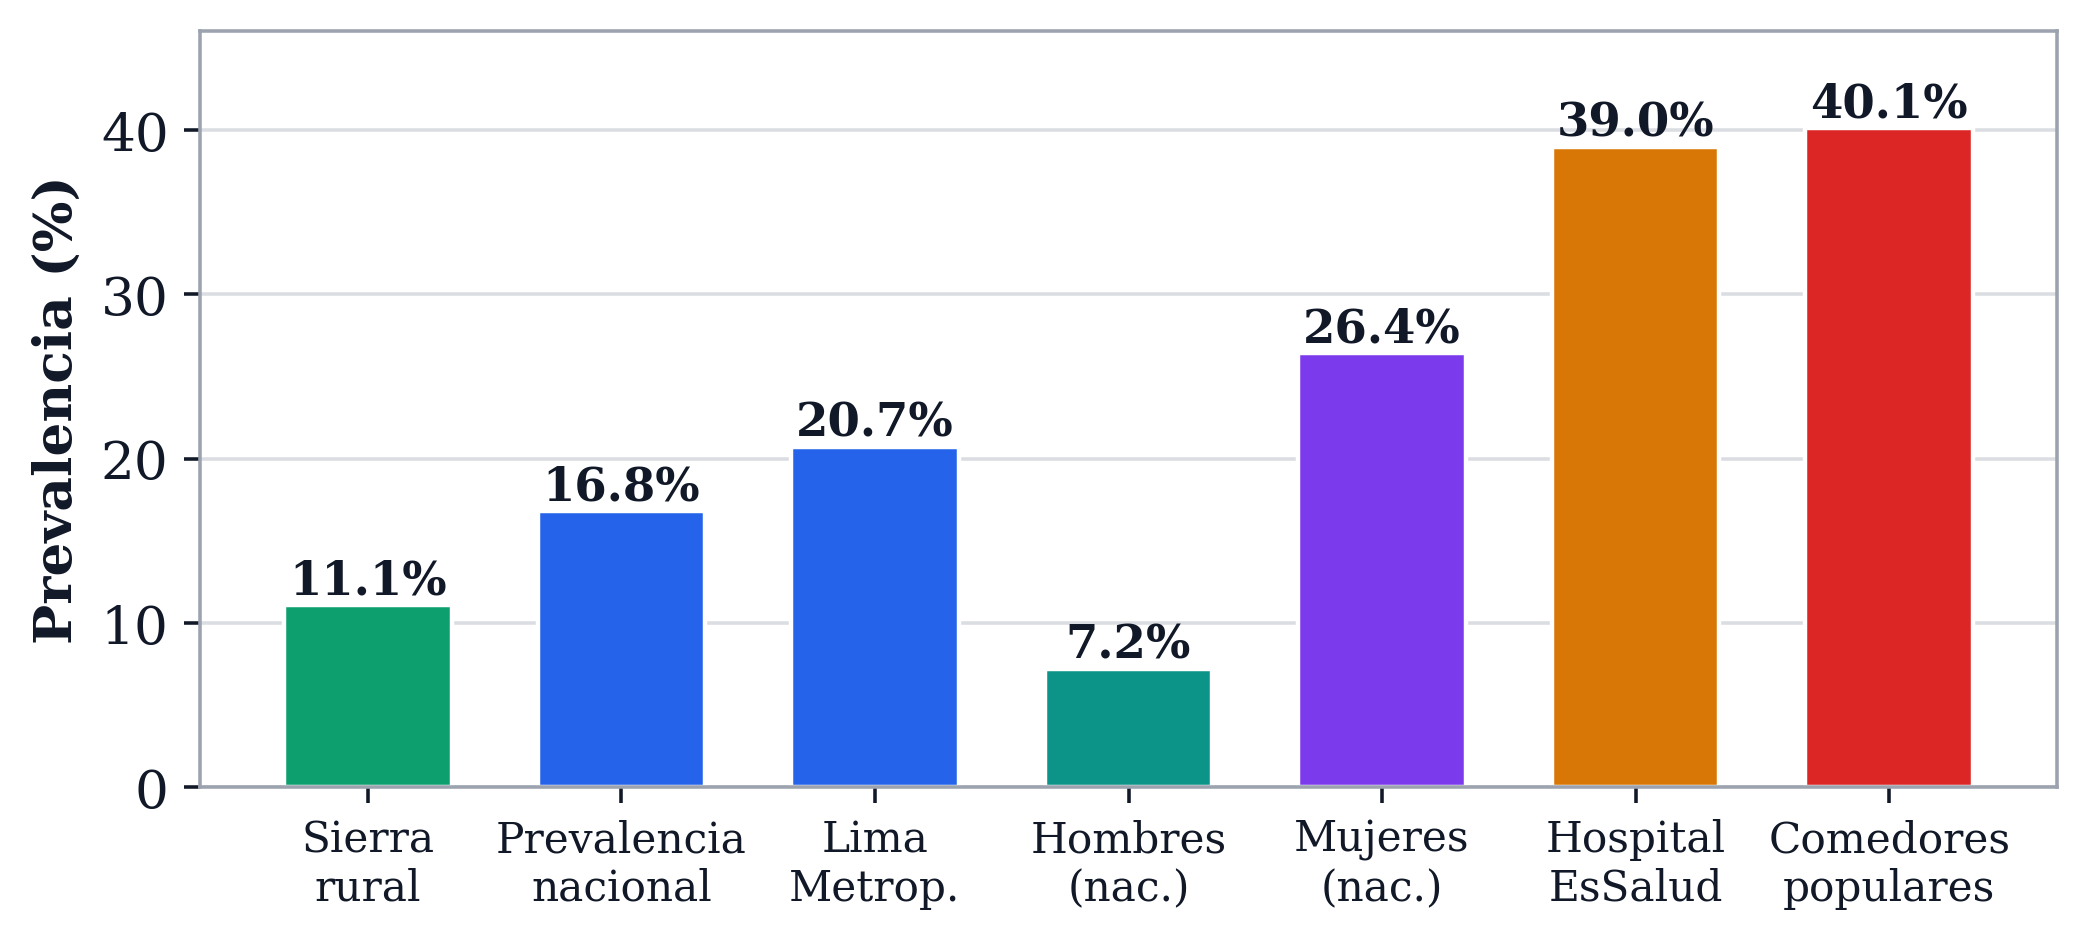
\includegraphics[width=\columnwidth]{fig_epi.png}
\caption{Prevalencia del síndrome metabólico en el Perú según población y
criterio diagnóstico. La asimetría de género y los picos en poblaciones
vulnerables justifican un tamizaje continuo, accesible y de bajo costo.}
\label{fig:epi}
\end{figure}

Frente a ese vacío proponemos \textbf{GEMA} (de ``Gemelo Metabólico''): un modelo
digital del metabolismo de cada persona que aprende de sus datos reales y estima
cómo responderá su cuerpo ante distintos hábitos, para devolverle
recomendaciones útiles en el momento. La idea de gemelo digital no es nueva en
salud, pero sí hay un hueco concreto que queremos llenar: no encontramos ninguna
herramienta de este tipo adaptada al contexto peruano ---la dieta de arroz, papa
y menú; el perfil del adulto limeño de 20 a 45 años; un módulo hormonal
femenino--- ni pensada para articularse con SIS y EsSalud.

El resto del artículo está organizado así. La Sección~\ref{sec:rel} ubica el
trabajo frente a la evidencia existente; la Sección~\ref{sec:met} describe la
arquitectura, el ICM, los datos con que entrenamos y los dos modelos; la
Sección~\ref{sec:res} reporta los resultados; la Sección~\ref{sec:app} presenta
la aplicación; y la Sección~\ref{sec:disc} discute alcances y limitaciones antes
de concluir.

%=============================================================================
\section{Trabajos Relacionados}\label{sec:rel}
%=============================================================================
Un gemelo digital en salud es, en esencia, una réplica computacional del
metabolismo de una persona que se mantiene al día integrando el sensor de
glucosa, los vestibles y los datos clínicos mediante aprendizaje automático. La
diabetes es un terreno fértil para este enfoque justamente porque es rico en
datos~\cite{oviedo}. La referencia obligada es \emph{Twin Health}, cuyo
``Whole Body Digital Twin'' reportó, en un ensayo controlado, una remisión de
diabetes tipo 2 del 71\,\% al cabo de un año, frente a apenas 2,4\,\% en la
atención estándar~\cite{twinhealth}. Ese resultado nos sirvió de prueba de que la
idea no es solo atractiva en el papel.

La pieza técnica que hace funcionar a estos sistemas es la \emph{respuesta
glucémica postprandial individual}: dos personas pueden comer exactamente el
mismo plato y registrar picos de glucosa muy distintos. Zeevi
\textit{et al.}~\cite{zeevi} mostraron que esa respuesta se puede anticipar con
\emph{gradient boosting} usando características de la comida y de la persona; es
precisamente el enfoque que adoptamos para nuestro Modelo~2. Para el índice
resumen nos inspiramos en los \emph{scores} continuos de severidad metabólica,
como el MetS-Z~\cite{gurka}, que demuestran que es viable condensar varios
marcadores en un solo número interpretable. GEMA toma estas ideas, las aterriza
al contexto local y las empaqueta en algo que cabe en un teléfono.

%=============================================================================
\section{Materiales y Métodos}\label{sec:met}
%=============================================================================
Organizamos el proyecto como un \emph{pipeline} reproducible que va desde la
captura del dato hasta la pantalla del usuario. La Fig.~\ref{fig:arq} resume la
arquitectura en cuatro capas; este artículo se concentra en la tercera (el motor
de IA) y en un MVP de la cuarta.

\begin{figure*}[t]
\centering
\resizebox{\textwidth}{!}{%
\begin{tikzpicture}[
  font=\footnotesize,
  layer/.style={rounded corners,draw=gink!30,thick,minimum height=1.45cm,
                inner sep=4pt,align=center},
  box/.style={rounded corners,draw=gink!35,fill=white,minimum height=0.95cm,
              minimum width=2.5cm,align=center,font=\scriptsize},
  arr/.style={-{Latex[length=2mm]},thick,gink!70}]
\node[layer,fill=gsoft, minimum width=4.0cm] (l1) {};
\node[box] (s1) at ($(l1.center)+(-1.05,0)$) {Sensor CGM\\(glucosa 5\,min)};
\node[box] (s2) at ($(l1.center)+(1.55,0.32)$) {Smartwatch BLE\\(HRV, pasos, sueño)};
\node[box] (s3) at ($(l1.center)+(1.55,-0.40)$) {App móvil\\(comidas, estrés)};
\node[above=1pt of l1,font=\scriptsize\bfseries\itshape] {1. Sensores / IoT};
\node[layer,fill=gsoft2,minimum width=4.0cm,right=1.0cm of l1] (l2) {};
\node[box] (b1) at ($(l2.center)+(0,0.32)$) {API Gateway + validación\\de rangos fisiológicos};
\node[box] (b2) at ($(l2.center)+(0,-0.42)$) {PostgreSQL +\\TimescaleDB};
\node[above=1pt of l2,font=\scriptsize\bfseries\itshape] {2. Ingesta / Backend};
\node[layer,fill=gsoft3,minimum width=4.6cm,right=1.0cm of l2] (l3) {};
\node[box,fill=gsoft] (m1) at ($(l3.center)+(0,0.34)$) {\textbf{Modelo 1}: riesgo\\(Random Forest)};
\node[box,fill=gsoft] (m2) at ($(l3.center)+(0,-0.42)$) {\textbf{Modelo 2}: pico\\glucémico (GBM)};
\node[above=1pt of l3,font=\scriptsize\bfseries\itshape] {3. Gemelo + Motor IA};
\node[layer,fill=gsoft4,minimum width=3.7cm,right=1.0cm of l3] (l4) {};
\node[box] (i1) at ($(l4.center)+(0,0.34)$) {App del paciente\\(avatar + ICM)};
\node[box] (i2) at ($(l4.center)+(0,-0.42)$) {Dashboard médico\\+ alertas};
\node[above=1pt of l4,font=\scriptsize\bfseries\itshape] {4. Interfaz};
\draw[arr] (l1)--(l2); \draw[arr] (l2)--(l3); \draw[arr] (l3)--(l4);
\end{tikzpicture}}
\caption{Arquitectura de GEMA en cuatro capas. El dato nace en los sensores y los
autorreportes, se valida y almacena en el backend, alimenta a los dos modelos del
gemelo y regresa al usuario convertido en un avatar, un índice de riesgo y
recomendaciones. El cumplimiento de la Ley N° 29733 de protección de datos
personales se aplica de extremo a extremo.}
\label{fig:arq}
\end{figure*}

\subsection{El Índice de Carga Metabólica (ICM)}
El ICM es la traducción del estado metabólico a un número de 0 a 100 que
cualquiera puede entender. Lo definimos como un promedio ponderado de cinco
sub-índices:
\begin{equation}
\text{ICM}=0{,}35\,g+0{,}20\,a+0{,}20\,s+0{,}15\,e+0{,}10\,n,
\label{eq:icm}
\end{equation}
donde $g,a,s,e,n\in[0,100]$ corresponden a glucosa, actividad, sueño, estrés y
nutrición. Los tramos 0--39 (verde), 40--69 (ámbar) y 70--100 (rojo) fijan el
color y la expresión del avatar (Fig.~\ref{fig:icm}). Que la glucosa pese más que
el resto no es arbitrario: es el marcador que el propio modelo de riesgo señala
como el más informativo, según veremos en la Sección~\ref{sec:res}. El usuario ve
este índice en la pantalla principal de la app (Fig.~\ref{fig:app}b), donde
además se desglosa en sus cinco componentes.

\begin{figure}[t]
\centering
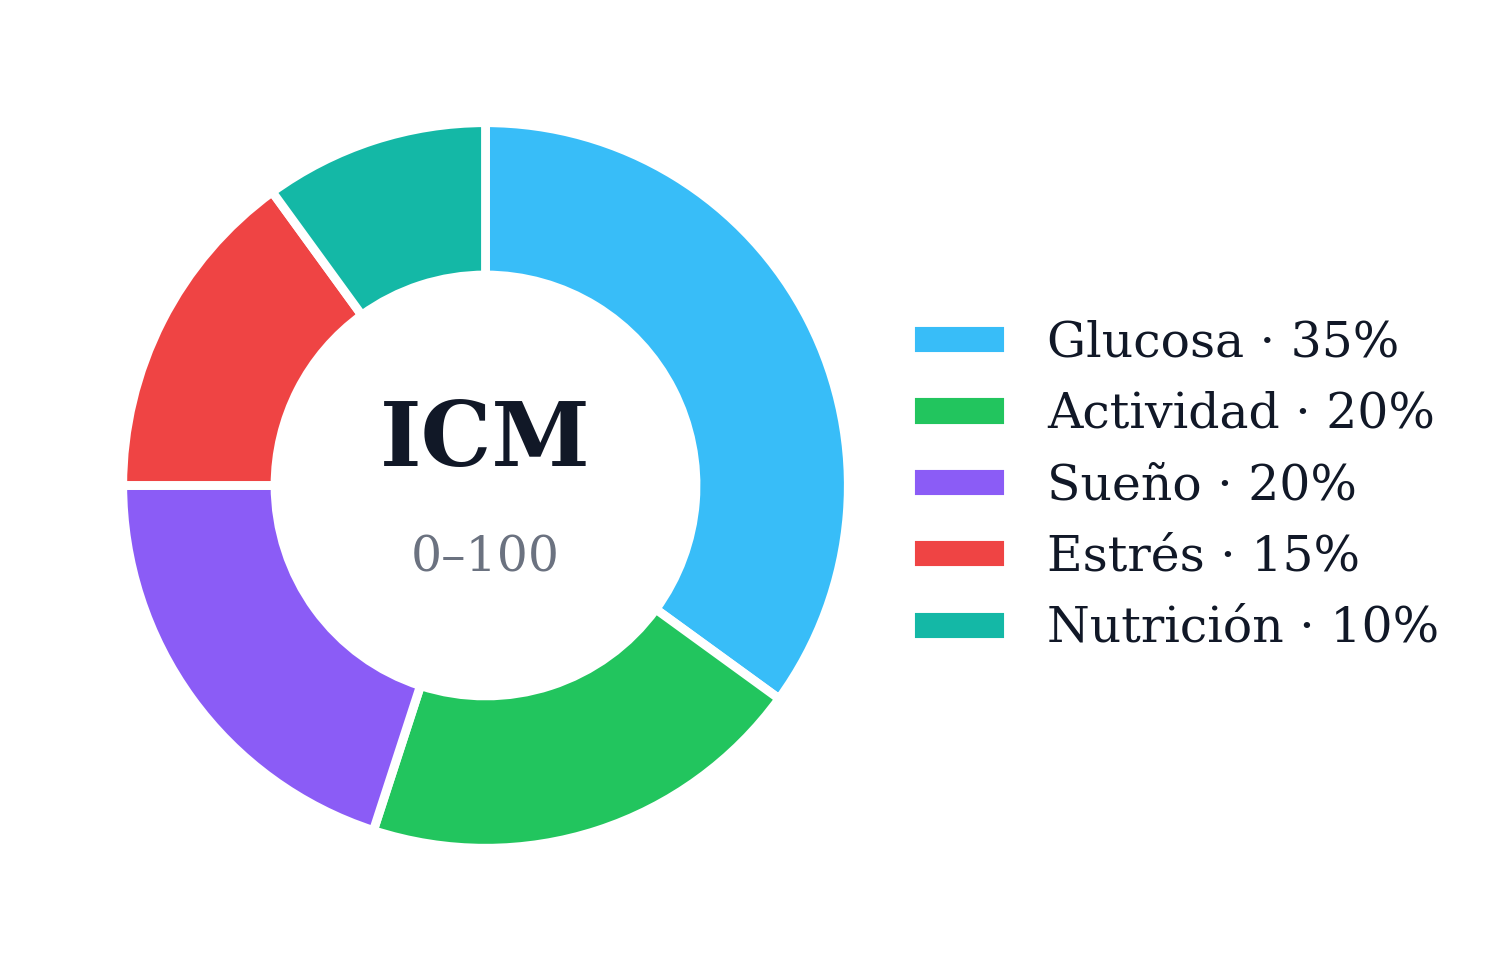
\includegraphics[width=0.92\columnwidth]{fig_icm.png}
\caption{Composición del Índice de Carga Metabólica. Cinco sub-índices ponderados
se condensan en un solo valor 0--100 que gobierna el estado del gemelo.}
\label{fig:icm}
\end{figure}

\subsection{Generación de la población de entrenamiento}
Aquí enfrentamos el obstáculo más evidente del proyecto: todavía no tenemos
usuarios reales con CGM, de modo que no hay un dataset propio con el cual
entrenar. En lugar de esperar, optamos por generar una población sintética
\emph{fisiológicamente plausible}: 6\,000 usuarios para el modelo de riesgo y
9\,000 eventos de comida para el de pico. La gracia no está en inventar números
al azar, sino en que esos números obedezcan relaciones causales que la literatura
ya documentó (Tabla~\ref{tab:fisio}). Por ejemplo, asignamos a cada usuario un
factor latente de ``carga metabólica'' y a partir de él derivamos sus hábitos y
marcadores, de manera que quien duerme poco tienda a mostrar más variabilidad
glucémica, y quien camina poco, más cintura. Sobre esa base añadimos ruido
individual para que el modelo aprenda patrones y no copias exactas.

\begin{table}[t]
\caption{Relaciones fisiológicas codificadas en el generador sintético}
\label{tab:fisio}
\centering
\footnotesize
\begin{tabularx}{\columnwidth}{@{}Xl@{}}
\toprule
\textbf{Relación modelada} & \textbf{Fuente}\\
\midrule
Carga glucémica $\to$ principal impulsor del pico & Zeevi 2015~\cite{zeevi}\\
Caminar tras comer $\to$ reduce el pico $\sim$20\,\% & Reynolds 2016~\cite{reynolds}\\
Dormir $<$7\,h $\to$ resistencia a insulina al día sig. & Spiegel 1999~\cite{spiegel}\\
HRV baja (estrés) $\to$ cortisol eleva la glucosa & NCEP/HPA~\cite{ncep}\\
Índice TyG $\to$ proxy de resistencia a la insulina & Simental 2008~\cite{tyg}\\
\bottomrule
\end{tabularx}
\end{table}

Validar el diseño fue tan importante como generarlo. Decidir distribuciones
realistas no garantiza que el problema sea aprendible, así que verificamos tres
cosas antes de entrenar. Primero, que las clases quedaran efectivamente
desbalanceadas, como ocurre en la realidad. Segundo, que ninguna variable
``filtrara'' la respuesta de forma trivial. Tercero, que la fuente de datos
pudiera intercambiarse sin tocar el resto del código: el día que lleguen datos
reales del piloto, solo cambia el origen, no el \emph{pipeline}. Este último
punto fue una decisión de ingeniería deliberada y, en la práctica, el principal
motivo por el que trabajamos con datos sintéticos en esta etapa.

\subsection{Modelo 1: clasificador de riesgo metabólico}
El primer modelo responde a una pregunta directa: ¿cómo está el usuario hoy? Lo
clasifica en riesgo bajo, moderado o alto y entrega la probabilidad de cada
clase, que la app usa para teñir y animar al gemelo. Es un \emph{Random Forest}
de 200 árboles que toma el resumen de los últimos 7 días en ocho variables
(Tabla~\ref{tab:vars}): variabilidad glucémica, tiempo en rango y pico
postprandial promedio del CGM; horas de sueño, pasos y HRV del reloj; índice TyG
de laboratorio; y circunferencia de cintura del perfil. Elegimos Random Forest
por tres motivos prácticos: tolera bien el ruido, captura interacciones no
lineales sin que tengamos que especificarlas, y ---no menos importante para una
herramienta de salud--- permite explicar en qué se apoya cada
decisión~\cite{breiman}.

\begin{table}[t]
\caption{Variables de entrada de los dos modelos de GEMA}
\label{tab:vars}
\centering
\footnotesize
\begin{tabularx}{\columnwidth}{@{}lX@{}}
\toprule
\textbf{Modelo} & \textbf{Variables de entrada (fuente)} \\
\midrule
\textbf{M1.} Riesgo & CV glucémico, tiempo en rango, pico postprandial
(CGM); sueño, pasos, HRV (smartwatch); índice TyG (laboratorio); cintura
(perfil) \\[2pt]
\textbf{M2.} Pico & Glucosa basal, carbohidratos, índice y carga glucémica
(comida); caminata posterior, sueño previo, HRV, hora del día \\
\bottomrule
\end{tabularx}
\end{table}

\subsection{Modelo 2: predictor del pico glucémico postprandial}
El segundo modelo mira hacia adelante: estima a cuánto subirá la glucosa
($\sim$60\,min después) si la persona come tal plato. Ese número es el que la app
muestra al registrar una comida. Lo resolvimos con un \emph{Gradient Boosting
Regressor} de 400 árboles alimentado por ocho variables del evento
(Tabla~\ref{tab:vars}): glucosa basal, carbohidratos, índice y carga glucémica
del plato, minutos de caminata posterior, sueño de la noche previa, HRV y hora
del día. Conviene aclarar que este modelo tabular es el \emph{baseline}: replica
el método de Zeevi \textit{et al.}~\cite{zeevi} y es el que entra al MVP. En
producción lo reemplazará una red LSTM que lea la serie completa del CGM de las
últimas 12\,h~\cite{oviedo}; dejamos esa puerta abierta a propósito.

%=============================================================================
\section{Resultados}\label{sec:res}
%=============================================================================
Evaluamos ambos modelos sobre conjuntos de prueba que el entrenamiento nunca vio
(20\,\% de los datos). La Tabla~\ref{tab:metrics} compara su desempeño con las
metas de la guía técnica; el resumen es que las dos quedan holgadamente cubiertas.

\begin{table}[t]
\caption{Desempeño de los modelos frente a las metas técnicas}
\label{tab:metrics}
\centering
\footnotesize
\begin{tabularx}{\columnwidth}{@{}lccc@{}}
\toprule
\textbf{Modelo / métrica} & \textbf{Resultado} & \textbf{Meta} & \textbf{Estado}\\
\midrule
M1 — Exactitud (test, $n{=}1200$)      & 88,5\,\%   & $>$85\,\%    & Cumple\\
M1 — Validación cruzada 5-fold         & 87,5$\pm$0,9\,\% & ---     & Cumple\\
M1 — F1 por clase (bajo/mod./alto)     & 0,90 / 0,85 / 0,91 & --- & Cumple\\
M2 — Error medio absoluto (MAE)        & 6,3\,mg/dL & $<$15\,mg/dL & Cumple\\
M2 — Coeficiente $R^2$ (test, $n{=}1800$) & 0,914   & ---          & Cumple\\
\bottomrule
\end{tabularx}
\end{table}

\subsection{Clasificación de riesgo}
El clasificador acertó el 88,5\,\% de los casos de prueba y se mantuvo estable en
validación cruzada (87,5\,\%$\pm$0,9\,\%), con F1 de 0,90, 0,85 y 0,91 para bajo,
moderado y alto. Más allá del promedio, lo que nos interesaba era \emph{cómo} se
equivoca, y ahí la matriz de confusión (Fig.~\ref{fig:conf}) trae una buena
noticia: el modelo nunca confunde un riesgo bajo con uno alto ni viceversa
---esas dos celdas son cero---; cuando falla, lo hace entre niveles vecinos, que
es el error menos grave para un tamizaje. El análisis de importancia de variables
(Fig.~\ref{fig:imp}) refuerza la coherencia clínica del modelo: el tiempo en
rango glucémico (29,1\,\%), la variabilidad de la glucosa (23,5\,\%) y el pico
postprandial (17,3\,\%) suman casi el 70\,\% de la decisión. Que los marcadores
del CGM manden de esa forma es justo lo que esperábamos, y es la razón empírica
detrás del peso de 0,35 que la glucosa recibe en la Ec.~\eqref{eq:icm}.

\begin{figure}[t]
\centering
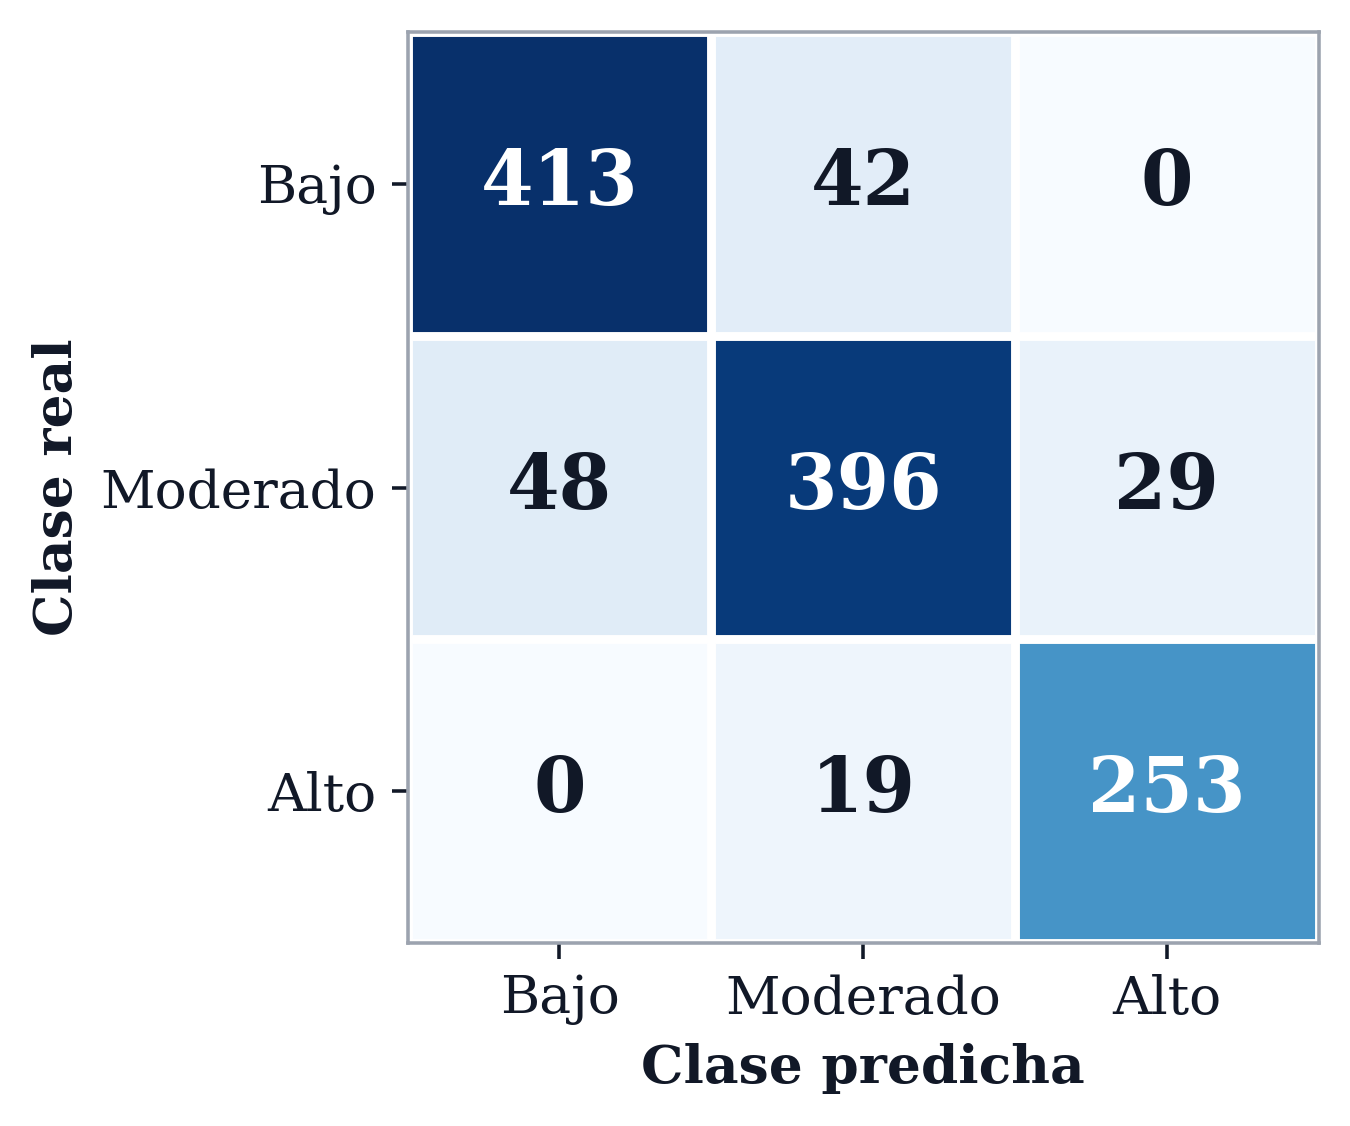
\includegraphics[width=0.86\columnwidth]{fig_confusion.png}
\caption{Matriz de confusión del clasificador sobre 1\,200 casos de prueba. La
masa se concentra en la diagonal y no hay cruces entre los extremos
bajo$\leftrightarrow$alto.}
\label{fig:conf}
\end{figure}

\begin{figure}[t]
\centering
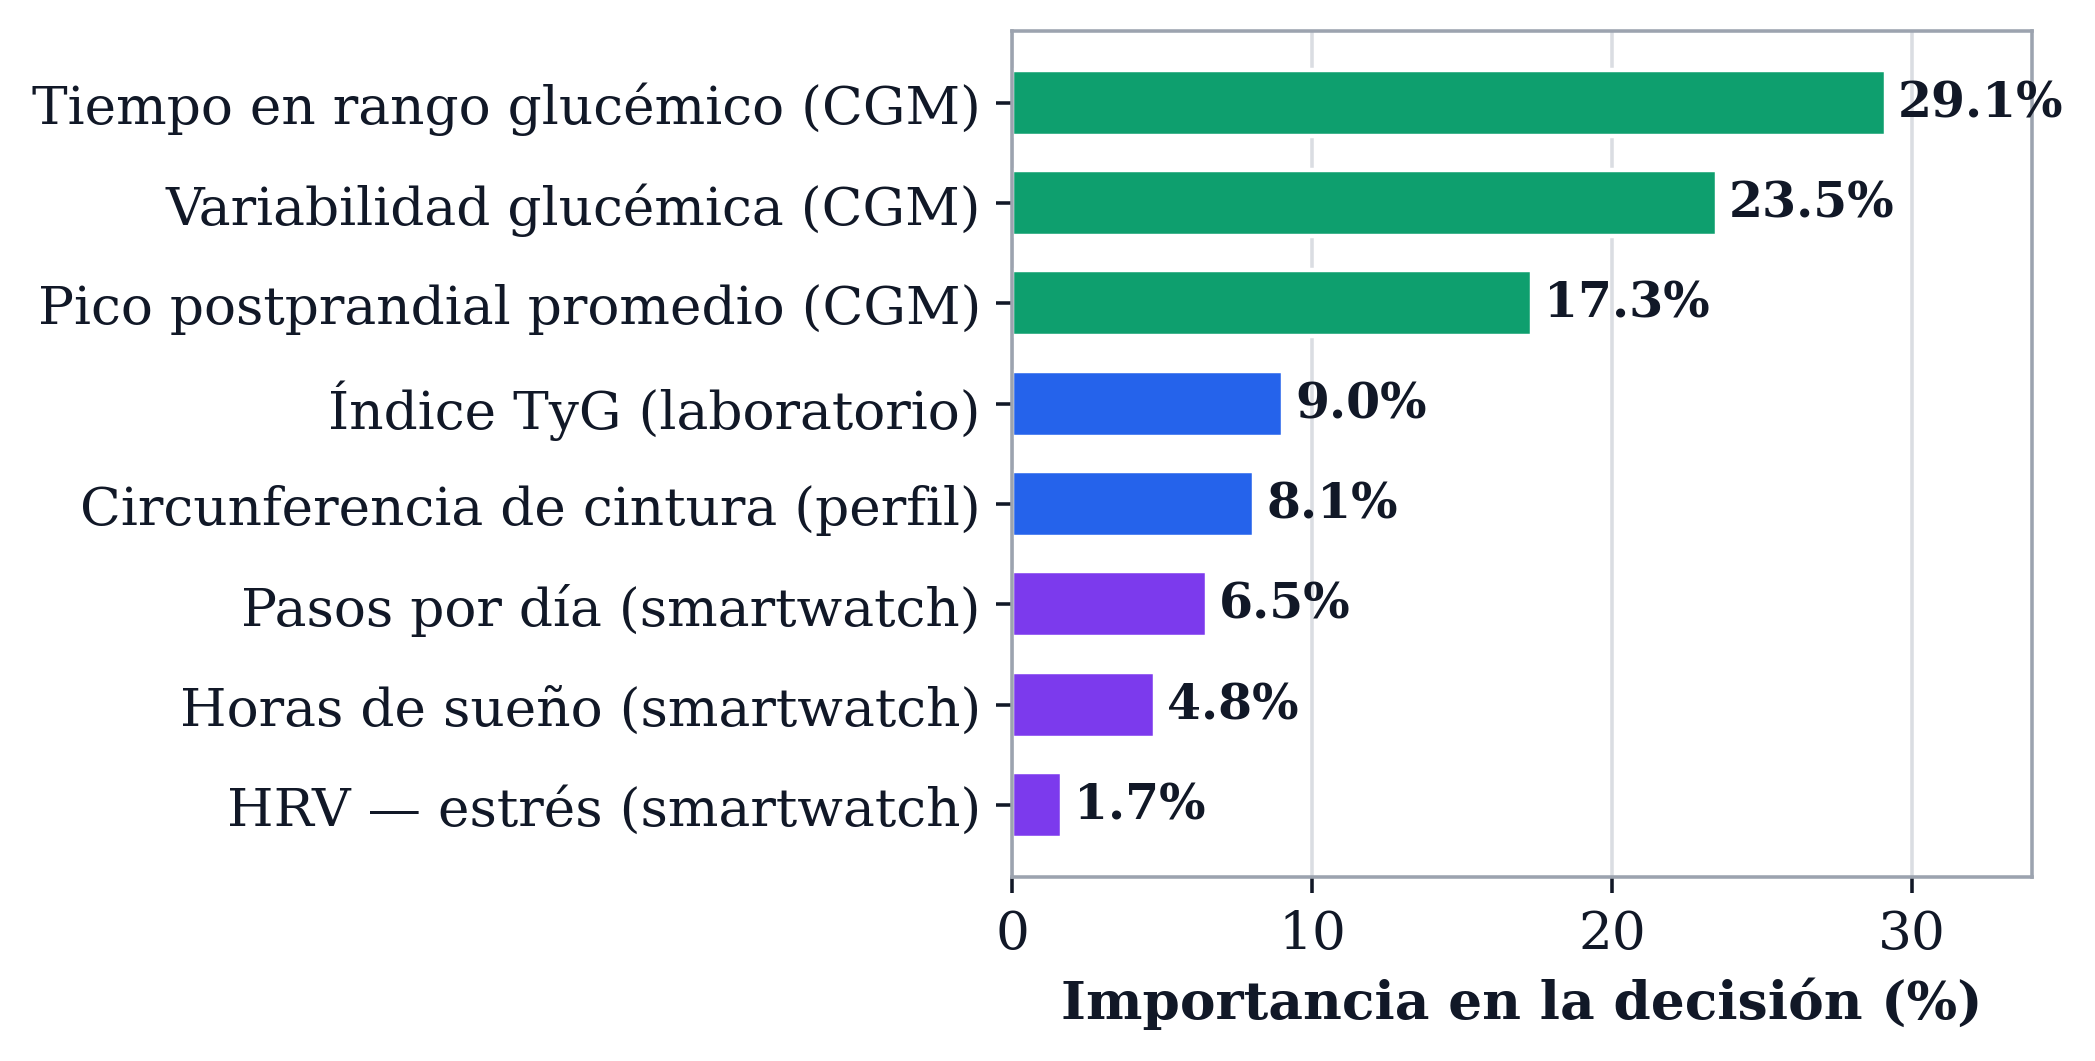
\includegraphics[width=\columnwidth]{fig_importancias.png}
\caption{Importancia de las variables en el clasificador de riesgo. Los
marcadores glucémicos del CGM concentran cerca del 70\,\% de la decisión.}
\label{fig:imp}
\end{figure}

\subsection{Predicción del pico glucémico}
El predictor de pico cerró con un error medio absoluto de 6,3\,mg/dL y un
$R^2=0{,}914$ sobre 1\,800 comidas de prueba. Para ponerlo en perspectiva, la
guía clínica considera aceptable un error de hasta 15\,mg/dL, así que nos
quedamos en menos de la mitad de ese margen. La Fig.~\ref{fig:pred} enfrenta lo
predicho con lo observado: la nube sigue de cerca la diagonal y la gran mayoría
de los puntos cae dentro de la banda de tolerancia.

\begin{figure}[t]
\centering
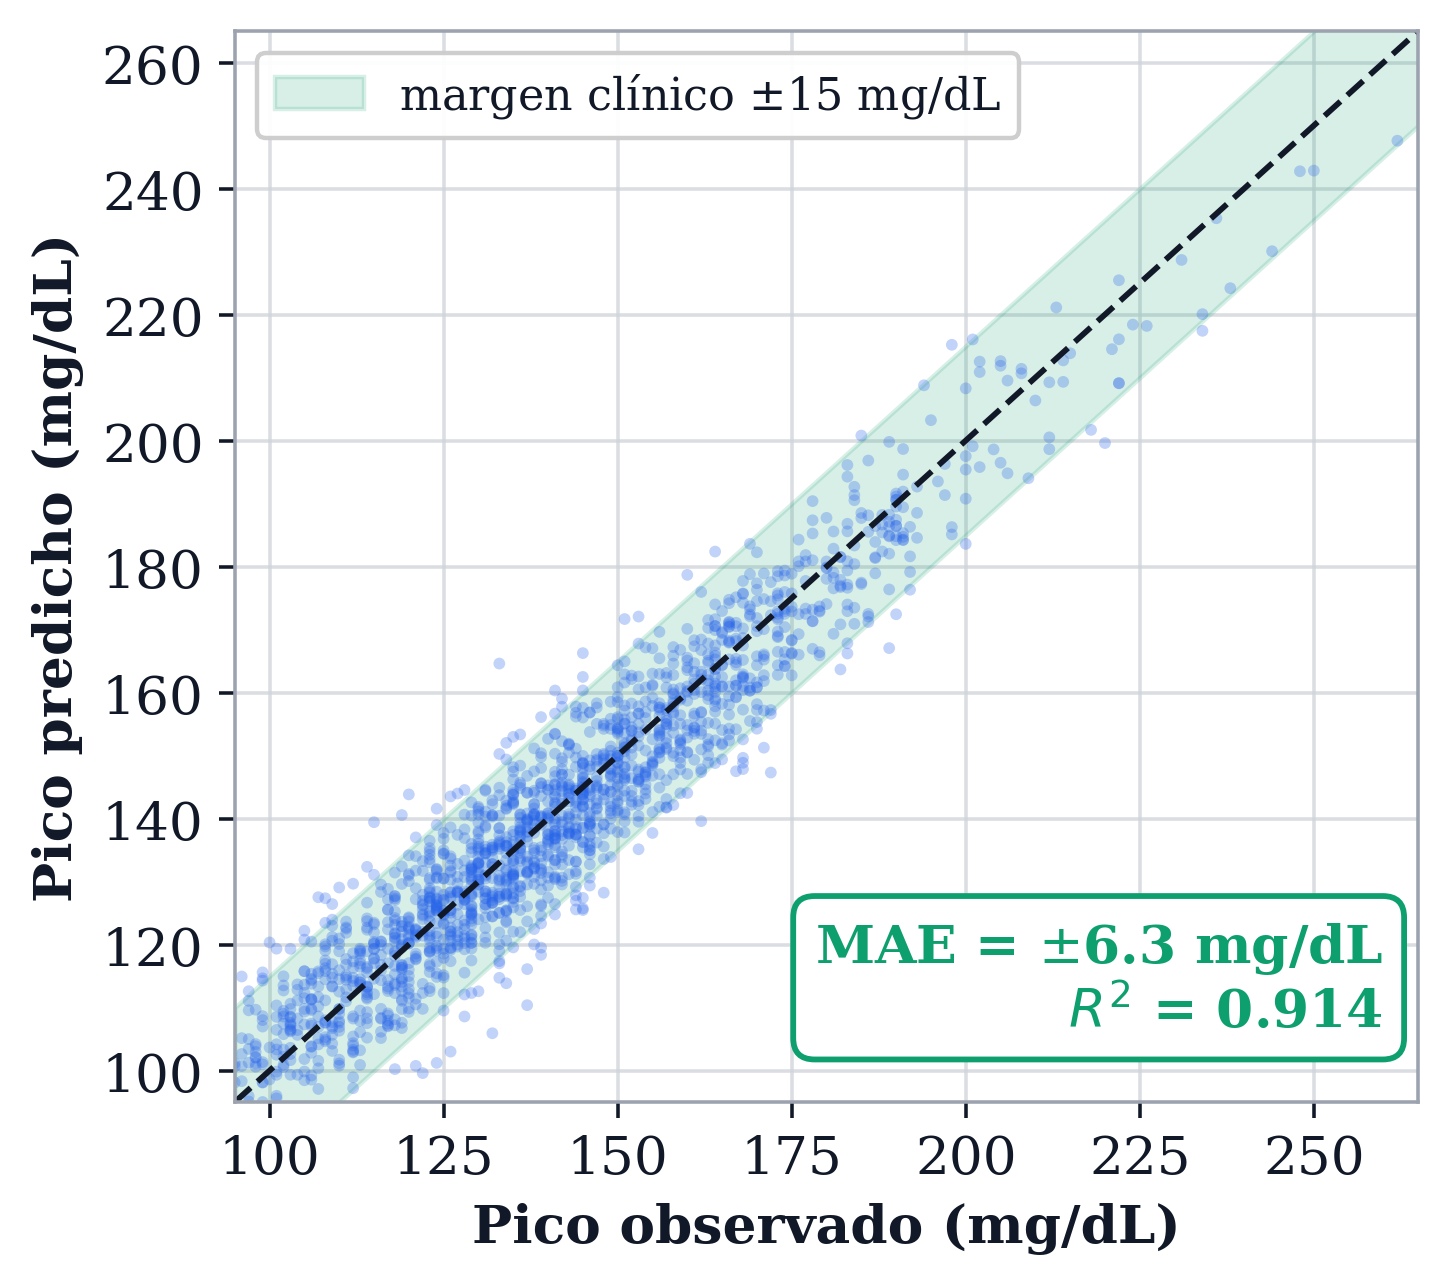
\includegraphics[width=0.92\columnwidth]{fig_pred_real.png}
\caption{Pico glucémico predicho frente al observado (1\,800 comidas de prueba).
Casi todos los puntos caen dentro de la banda clínica de $\pm$15\,mg/dL.}
\label{fig:pred}
\end{figure}

\subsection{Del pronóstico a la recomendación}
Un buen pronóstico, por sí solo, no cambia hábitos. Por eso lo que de verdad
explotamos del Modelo~2 es su capacidad de responder preguntas
contrafactuales. El simulador toma una comida concreta, la evalúa bajo varias
decisiones posibles y se queda con la que más baja el pico. La
Fig.~\ref{fig:whatif} ilustra el caso de un almuerzo muy peruano ---arroz con
pollo, 78\,g de carbohidratos, índice glucémico 72--- en alguien que durmió solo
5,7\,h. Sin intervenir, el modelo prevé un pico de 164\,mg/dL, claramente alto.
Caminar 25\,min lo baja a 149; cambiar el arroz por quinua, a 150; y hacer las
dos cosas juntas lo lleva a 132\,mg/dL, ya dentro de rango. De esa comparación
nacen, literalmente, los dos consejos que la app le muestra al usuario. Es la
diferencia entre decirle ``tu glucosa está alta'' y decirle ``camina 25 minutos
y cambia el arroz por quinua''.

\begin{figure}[t]
\centering
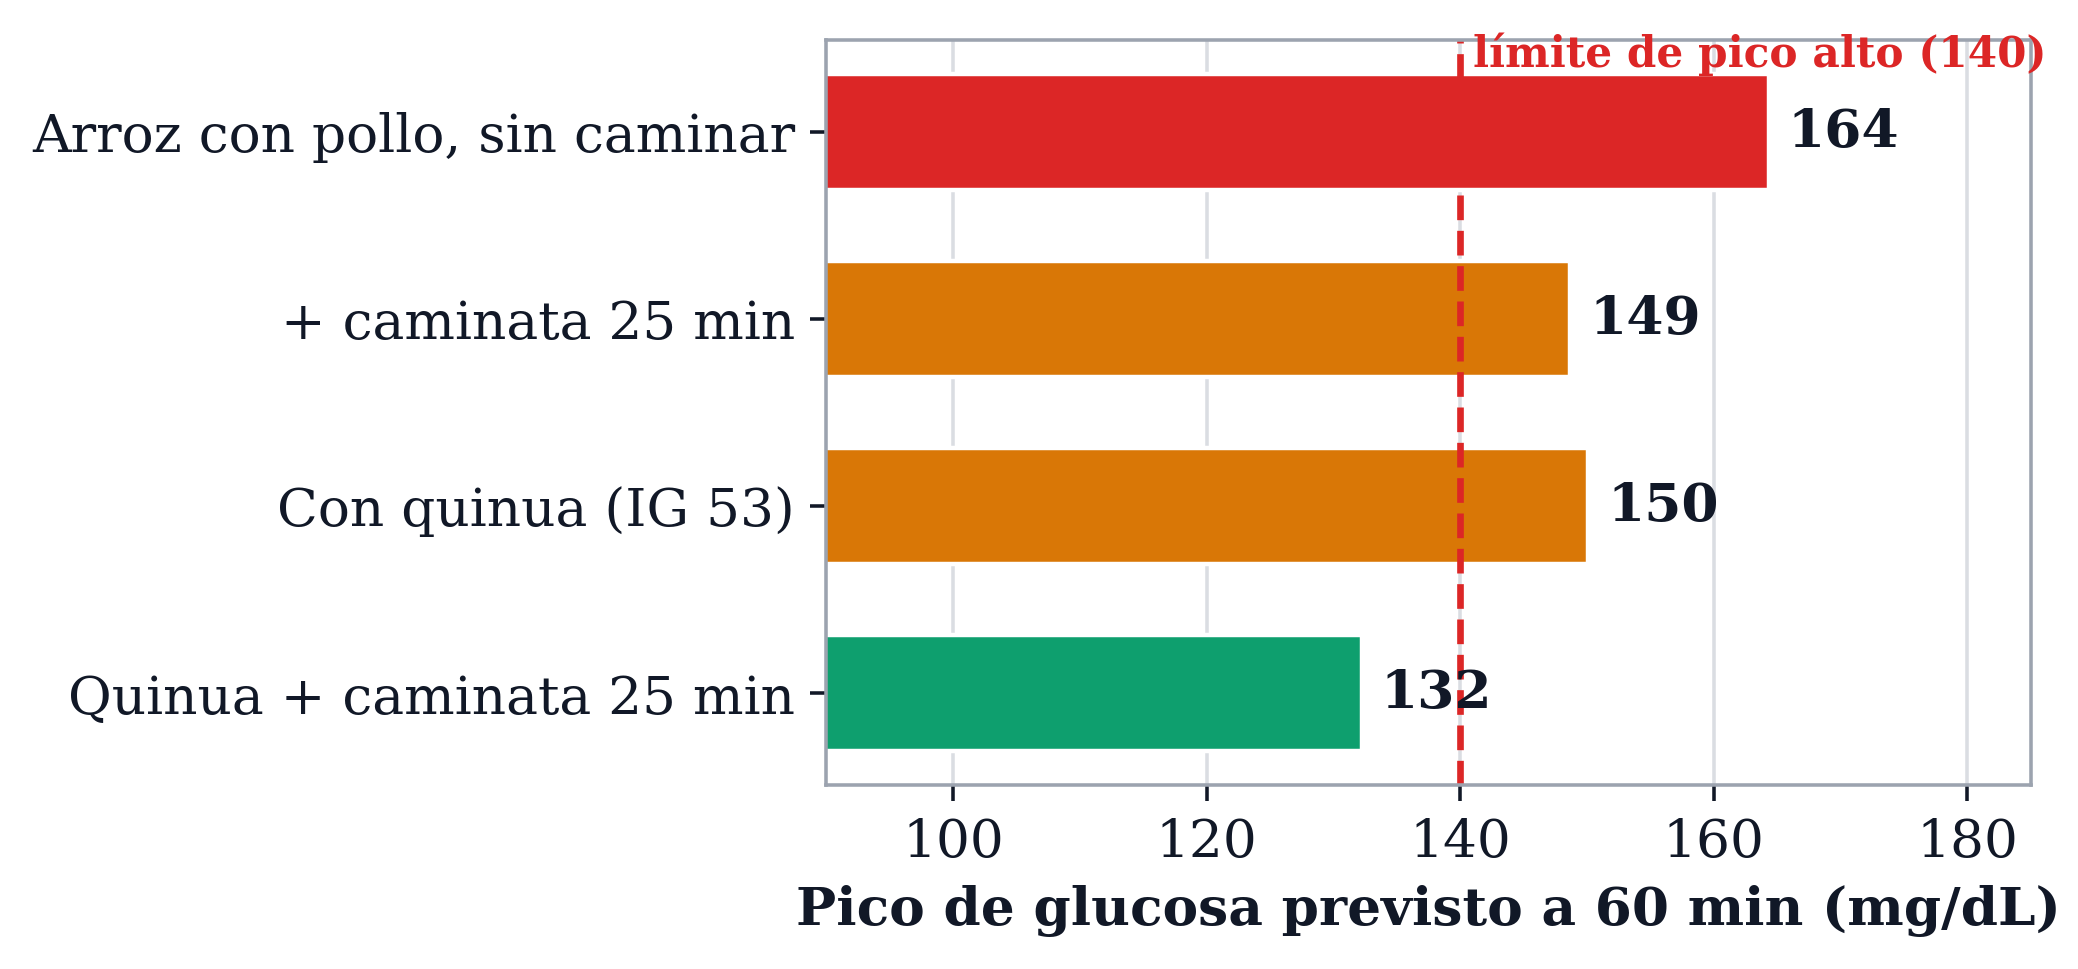
\includegraphics[width=\columnwidth]{fig_whatif.png}
\caption{Simulación contrafactual para un mismo almuerzo bajo cuatro decisiones.
Quinua más caminata recorta el pico 32\,mg/dL, de 164 (alto) a 132 (rango
saludable).}
\label{fig:whatif}
\end{figure}

%=============================================================================
\section{La Aplicación (MVP)}\label{sec:app}
%=============================================================================
El gemelo cobra forma en una aplicación móvil construida con Next.js y React,
con 14 pantallas navegables. La Fig.~\ref{fig:app} muestra dos de ellas. La de
bienvenida (a) plantea desde el inicio el contrato con el usuario: acceso con
Google o correo y, al pie, el aviso de cumplimiento de la Ley N° 29733 y el
cifrado AES-256. La pantalla principal (b) es el corazón de la experiencia:
presenta el ICM del día ---en el ejemplo, 60, ``riesgo moderado''--- junto al
gemelo y al desglose de los cinco sub-índices, cada uno con su valor y su
tendencia.

\begin{figure}[t]
\centering
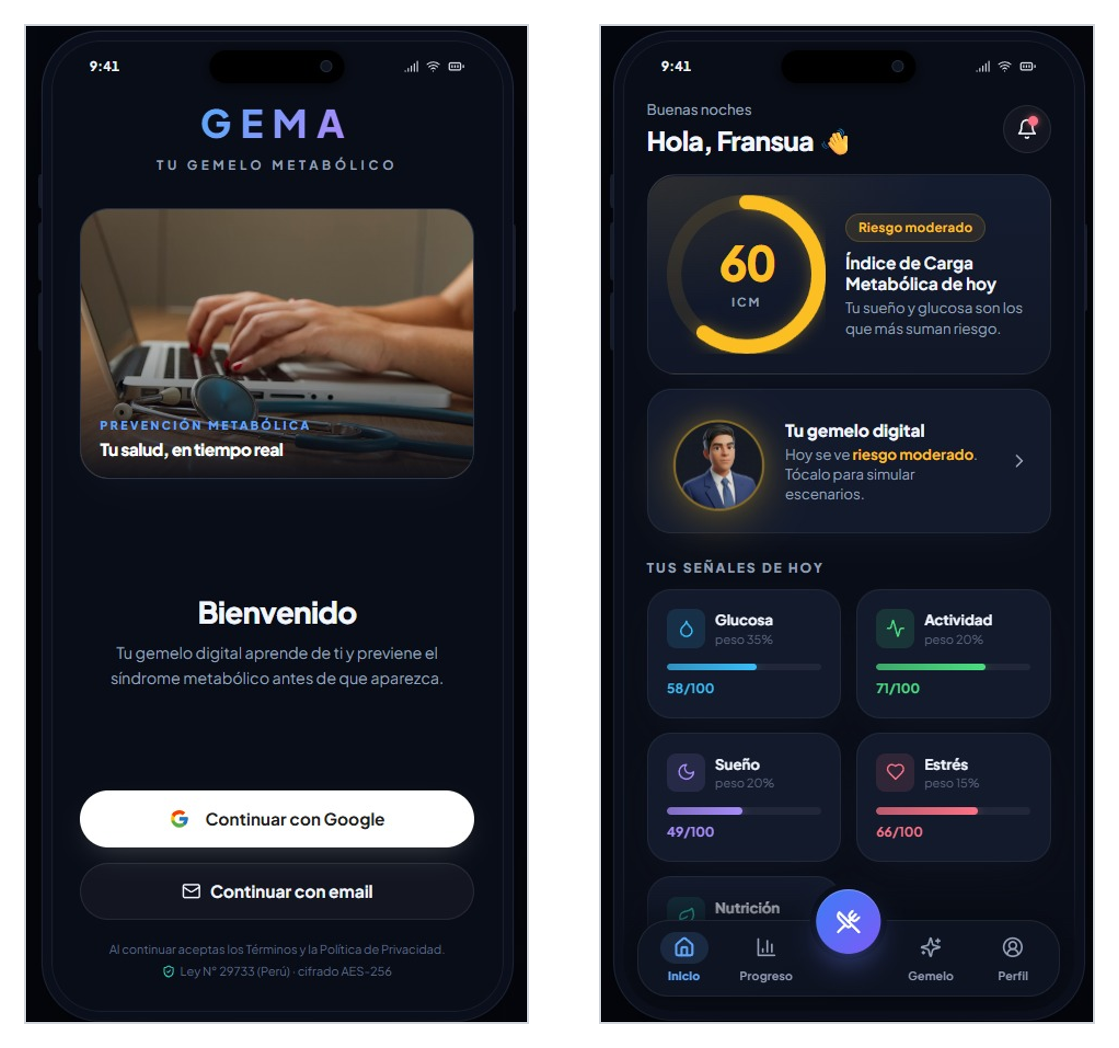
\includegraphics[width=0.96\columnwidth]{fig_app.png}
\caption{Capturas reales del MVP. (a)~Bienvenida con login y aviso de privacidad
(Ley N° 29733, cifrado AES-256). (b)~Panel principal con el ICM del día, el
gemelo y los cinco sub-índices.}
\label{fig:app}
\end{figure}

El elemento que mejor comunica el estado de salud no es una cifra sino el propio
avatar, que cambia de gesto, color y postura según el ICM
(Fig.~\ref{fig:twin}): sonríe y se ve enérgico cuando el riesgo es bajo, se torna
neutro cuando es moderado y luce cansado cuando es alto. Apostamos por esta
metáfora porque convierte un dato clínico abstracto en una señal emocional que se
capta de un vistazo, sin necesidad de interpretar números.

\begin{figure}[t]
\centering
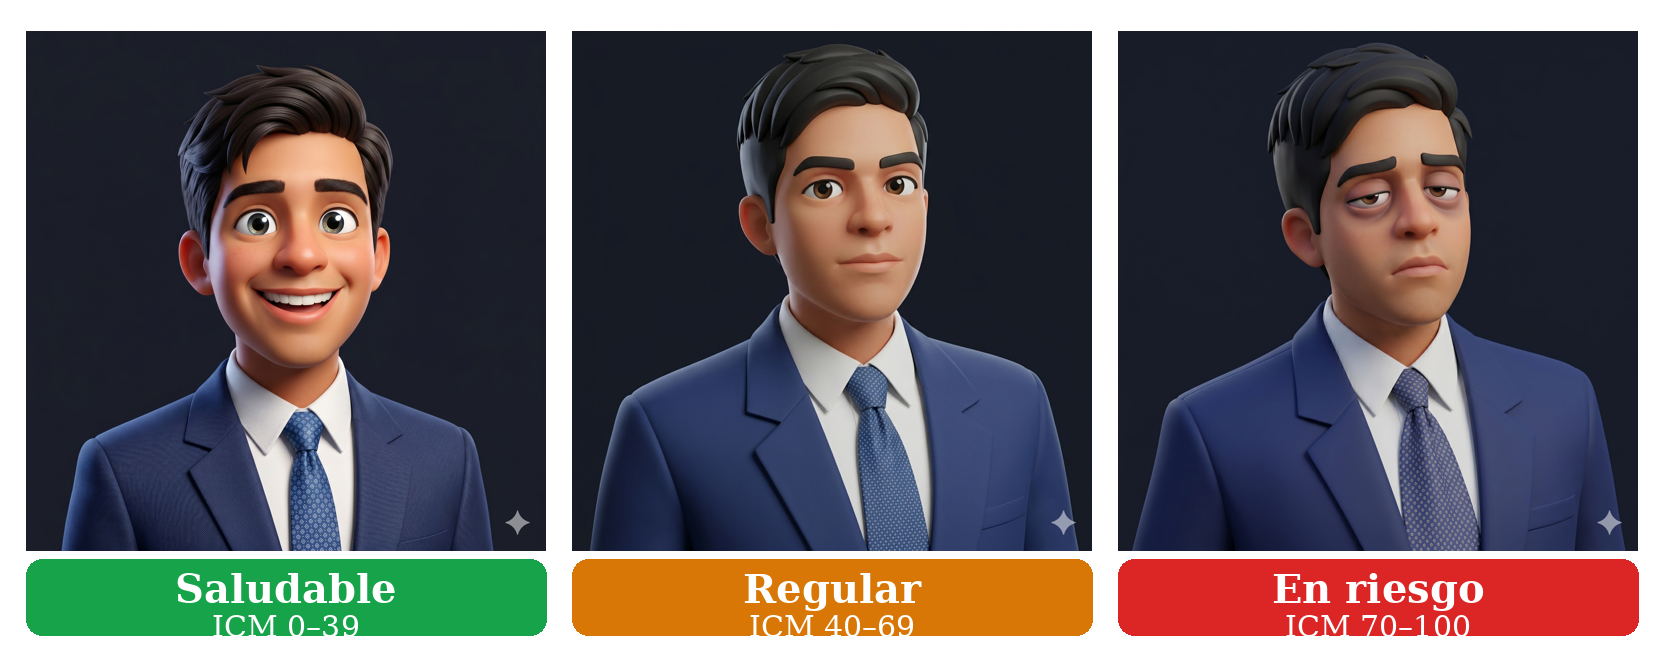
\includegraphics[width=\columnwidth]{fig_twin.png}
\caption{El gemelo reacciona en tiempo real al ICM: expresión, color y postura
comunican el nivel de riesgo (bajo, moderado, alto) de un solo vistazo.}
\label{fig:twin}
\end{figure}

Las demás pantallas acompañan el ciclo completo de uso, agrupadas en cuatro
bloques (Tabla~\ref{tab:screens}): el \emph{onboarding}, el núcleo de monitoreo
diario, el seguimiento a mediano plazo y el puente con el sistema de salud. Dos
capacidades ya son reales, no simuladas: el análisis del plato por visión por
computador ---que estima carbohidratos, índice y carga glucémica desde una foto y
alimenta al Modelo~2--- y el simulador ``¿qué pasaría si\ldots?'', que recalcula
el ICM y el pico en vivo al mover los controles. El resto de integraciones de
hardware (smartwatch BLE y sensor CGM) son, por ahora, \emph{mocks} a la espera
del piloto.

\begin{table}[t]
\caption{Las 14 pantallas del MVP, agrupadas por etapa de uso}
\label{tab:screens}
\centering
\footnotesize
\begin{tabularx}{\columnwidth}{@{}lX@{}}
\toprule
\textbf{Bloque} & \textbf{Pantallas}\\
\midrule
Onboarding   & Bienvenida y login, crear gemelo (cámara), personalizar gemelo, procesando \\[2pt]
Núcleo       & Panel principal (ICM), mi gemelo + simulador, registro diario de comida / sueño / estrés \\[2pt]
Seguimiento  & Progreso e historial, proyección de riesgo a 5 años, recomendaciones, alertas, detalle de sub-índice \\[2pt]
Clínico      & Reporte para el médico, perfil del usuario \\
\bottomrule
\end{tabularx}
\end{table}

\subsection{Privacidad y cumplimiento}
Tratándose de datos de salud, la privacidad no fue un agregado de última hora
sino un requisito de diseño. GEMA se construye para cumplir la Ley N° 29733 de
Protección de Datos Personales del Perú: el consentimiento se solicita en la
misma pantalla de bienvenida (Fig.~\ref{fig:app}a), la información viaja cifrada
con TLS 1.3 y se almacena con AES-256, y el backend valida que cada lectura caiga
dentro de rangos fisiológicos antes de guardarla ---lo que, de paso, descarta
errores de los sensores. El público al que apuntamos primero son los adultos de
20 a 45 años de Lima Metropolitana con dos o más alteraciones metabólicas, un
segmento donde la detección temprana rinde más y que conecta de forma natural con
la cobertura de SIS y EsSalud.

%=============================================================================
\section{Discusión y Limitaciones}\label{sec:disc}
%=============================================================================
Conviene ser claros sobre el alcance de estos resultados. La limitación de fondo
es que los modelos se entrenaron con datos sintéticos: las métricas demuestran
que el \emph{pipeline} funciona y que las relaciones fisiológicas asumidas son
aprendibles, pero no equivalen todavía a una validación clínica. Un riesgo
asociado es que el modelo aprenda las reglas que nosotros mismos codificamos en
el generador; lo mitigamos con ruido individual y comprobaciones de variedad,
aunque la prueba definitiva solo llegará con datos reales.

El plan para cerrar esa brecha tiene tres pasos. El primero es un piloto con
usuarios reales y dos semanas de calibración por persona, que permitiría afinar
el gemelo de forma individual. El segundo es sustituir el Gradient Boosting por
la red LSTM prevista, capaz de aprovechar la dinámica temporal del CGM en lugar
de un resumen tabular. El tercero es preentrenar el modelo base con datasets
poblacionales de referencia como NHANES y ENDES, y reentrenar de forma periódica.
Quedan también frentes abiertos que excedían este entregable: el módulo hormonal
femenino, la integración formal con SIS y EsSalud, y un estudio de generalización
fuera de Lima.

Aun con estas salvedades, el potencial de impacto justifica seguir adelante. En
el país, entre el 40\,\% y el 60\,\% de las amputaciones no traumáticas se deben
a la diabetes, y la mortalidad por esta causa creció más de 50\,\% en dos
décadas; muchos pacientes debutan directamente con un infarto. Una herramienta
que adelante la detección y sostenga el seguimiento ataca justo el tramo del
problema donde hoy no hay nadie acompañando al paciente. No es casual que el
mercado de gemelos digitales en salud, valorado en USD 4,92\,mil millones en
2024, se proyecte hacia los USD 21,3\,mil millones para 2032: la evidencia y la
demanda apuntan en la misma dirección.

%=============================================================================
\section{Conclusiones}
%=============================================================================
\begin{itemize}[leftmargin=1.1em,itemsep=2pt,topsep=2pt]
\item El clasificador de riesgo alcanzó 88,5\,\% de exactitud (87,5\,\% en
validación cruzada), por encima de la meta de 85\,\%, y ---lo más relevante en
salud--- no comete el error grave de confundir riesgo bajo con alto. Sus
decisiones se apoyan en marcadores glucémicos del CGM, que reúnen cerca del
70\,\% de la importancia.
\item El predictor de pico erró en promedio 6,3\,mg/dL ($R^2=0{,}91$), menos de
la mitad del margen clínico de 15\,mg/dL, y habilita un simulador que cuantifica
el efecto de caminar o de cambiar un alimento.
\item El ICM y el avatar logran traducir un estado clínico complejo en una señal
que cualquiera entiende, y el MVP de 14 pantallas demuestra que la experiencia
de usuario completa es viable hoy.
\item En conjunto, GEMA ataca la causa de fondo ---la falta de detección
temprana y de seguimiento--- con una herramienta de bajo costo y pensada para el
contexto peruano, y deja un \emph{pipeline} reproducible listo para recibir datos
reales en la fase piloto.
\end{itemize}

%=============================================================================
\section*{Reconocimientos}
%=============================================================================
\small
Agradecemos a los docentes de la Facultad de Ingeniería Industrial y de Sistemas
de la UNI por su retroalimentación durante el desarrollo del proyecto. El código
del modelo predictivo y de la aplicación se entrega junto a este informe.

%=============================================================================
\begin{thebibliography}{99}
\footnotesize
\bibitem{ncep} National Cholesterol Education Program (NCEP-ATP III) and
AHA/NHLBI, ``Diagnosis and management of the metabolic syndrome,''
\textit{Circulation}, vol.~112, no.~17, pp.~2735--2752, 2005.
\bibitem{prevperu} Instituto Nacional de Estadística e Informática y SciELO
Perú, ``Prevalencia de síndrome metabólico en adultos peruanos (criterio
ATP~III),'' \textit{Rev. Peruana de Medicina Experimental y Salud Pública},
2018.
\bibitem{comedores} L. Pajuelo \textit{et al.}, ``Síndrome metabólico en
usuarios de comedores populares de Lima,'' \textit{Rev. Peruana de Medicina
Experimental y Salud Pública}, 2019.
\bibitem{zeevi} D. Zeevi \textit{et al.}, ``Personalized nutrition by prediction
of glycemic responses,'' \textit{Cell}, vol.~163, no.~5, pp.~1079--1094, 2015.
\bibitem{twinhealth} P. Shamanna \textit{et al.}, ``Reducing HbA1c in type~2
diabetes using digital twin technology-enabled precision nutrition,''
\textit{Diabetes Therapy}, vol.~11, pp.~2703--2714, 2020.
\bibitem{reynolds} A. N. Reynolds \textit{et al.}, ``Advice to walk after meals
is more effective for lowering postprandial glycaemia,'' \textit{Diabetologia},
vol.~59, pp.~2572--2578, 2016.
\bibitem{spiegel} K. Spiegel, R. Leproult, and E. Van Cauter, ``Impact of sleep
debt on metabolic and endocrine function,'' \textit{The Lancet}, vol.~354,
pp.~1435--1439, 1999.
\bibitem{tyg} L. E. Simental-Mendía \textit{et al.}, ``The product of fasting
glucose and triglycerides as surrogate for insulin resistance,'' \textit{Metab.
Syndr. Relat. Disord.}, vol.~6, no.~4, pp.~299--304, 2008.
\bibitem{gurka} M. J. Gurka \textit{et al.}, ``An examination of sex and
racial/ethnic differences in the metabolic syndrome severity score,''
\textit{Metabolism}, vol.~63, no.~2, pp.~218--225, 2014.
\bibitem{breiman} L. Breiman, ``Random forests,'' \textit{Machine Learning},
vol.~45, no.~1, pp.~5--32, 2001.
\bibitem{oviedo} S. Oviedo \textit{et al.}, ``A review of personalized blood
glucose prediction strategies for T1DM patients,'' \textit{Int. J. Numer.
Method Biomed. Eng.}, vol.~33, no.~6, 2017.
\bibitem{idf} International Diabetes Federation, \textit{IDF Diabetes Atlas},
10th ed., Brussels, Belgium, 2024. [Online]. Available:
\url{https://diabetesatlas.org/}
\bibitem{geron} A. Géron, \textit{Hands-On Machine Learning with Scikit-Learn,
Keras and TensorFlow}, 2nd ed. Sebastopol, CA: O'Reilly, 2019.
\end{thebibliography}

\end{document}
